\documentclass[11pt]{article}
 \usepackage{geometry}
 \geometry{letterpaper, top=1.2in, bottom=1.2in, left=1in, right=1in}
\usepackage{verbatim}
\usepackage[rgb]{xcolor}
\usepackage{tikz}
\usetikzlibrary{shapes,snakes,calendar,matrix,backgrounds,folding}
\usepackage{graphicx}
\usepackage{epsfig}
\usepackage{alltt}
\usepackage{amsmath}
\usepackage{epsfig}
\usepackage{amssymb,amsfonts,epsf,url}
\usepackage{pstricks,pstricks-add}
\usepackage{pst-coil}
\usepackage{pst-node}
\usepackage{clrscode}


\usepackage{fancyhdr}




\newcommand{\important}[2] {\node[name=#1, minimum size=8mm] {#2};}
\newcommand{\leaf}[2] {\node[rectangle,name=#1, minimum size=5mm] {#2};}
\newcommand{\uncle}[2] {\node[name=#1, gray] {#2};}
\newcommand{\othernode}[2] {\node[name=#1, fill=none] {#2};}
\renewcommand{\labelenumi}{\arabic{enumi}.}
\renewcommand{\labelenumii}{\arabic{enumi}.\arabic{enumii}.}
\renewcommand{\labelenumiii}{\arabic{enumi}.\arabic{enumii}.\arabic{enumiii}.}
\renewcommand{\labelenumiv}{\arabic{enumi}.\arabic{enumii}.\arabic{enumiii}.\arabic{enumiv}.}
\newlength{\alginputwidth}
\newlength{\algboxwidth}
\newcommand{\alginput}[1]{\makebox[1.5cm][l]{ {\sc Input:}} \parbox[t]{\alginputwidth}{{\it #1}}}
\newcommand{\algoutput}[1]{\makebox[1.5cm][l]{ {\sc Output:}} \parbox[t]{\alginputwidth}{{\it #1}}}
\newcommand{\algtitle}[1]{\underline{Algorithm \ {\bf #1}} \vspace*{1mm}\\}

\newsavebox{\algbox}
\newsavebox{\captionbox}
\newenvironment{algorthm}[2]{
        \setlength{\algboxwidth}{\columnwidth}
        \addtolength{\algboxwidth}{-\columnsep}
        \addtolength{\algboxwidth}{-1mm}
        \setlength{\alginputwidth}{\algboxwidth}
        \addtolength{\alginputwidth}{-1.7cm}
        \begin{figure}[tb]
            \vspace*{2mm}
            \centering
            \begin{lrbox}{\captionbox}
                \begin{minipage}[b]{\algboxwidth}
                    \centering
                    \caption{#1}
                    \label{#2}
                \end{minipage}
            \end{lrbox}
            \begin{lrbox}{\algbox}
                \begin{minipage}[b]{\algboxwidth}
                    \footnotesize
                    \vspace*{2mm}
    } {
                    \vspace*{0.2mm}
               \end{minipage}
            \end{lrbox}
            \fbox{\usebox{\algbox}\hspace*{1mm}}
            \usebox{\captionbox}
            \vspace*{-4mm}
        \end{figure}
    }
\newsavebox{\algcodebox}
\newenvironment{codeblock}{
        \begin{enumerate}
            \setlength{\itemsep}{2pt}
            \setlength{\parsep}{0pt}
            \setlength{\topsep}{0pt}
            \setlength{\parskip}{0pt}
            \setlength{\partopsep}{0pt}
    } {\end{enumerate}}



\newcommand{\paramproblem}[4]{\noindent {\sc #1}
\\
{\bf Given:} #2\\
{\bf Parameter:} #3\\
{\bf Question:} #4}


\newcommand{\YES}{\textup{\textsf{YES}}}
\newcommand{\NO}{\textup{\textsf{NO}}}
\newcommand{\Oh}{{\mathcal O}}
\newcommand{\nat}{\mathbb{N}}

\newcommand{\Pol}{\mbox{}}
\newcommand{\NP}{\mbox{}}


\newtheorem{theorem}{Theorem}[section]
\newtheorem{lemma}[theorem]{Lemma}
\newtheorem{claim}[theorem]{Claim}
\newtheorem{corollary}[theorem]{Corollary}
\newtheorem{proposition}[theorem]{Proposition}
\newtheorem{observation}[theorem]{Observation}
\newtheorem{reduction}{Reduction Rule}[section]
\newtheorem{operation}{Operation}[section]
\newtheorem{fact}[theorem]{Fact}
\newtheorem{case}[theorem]{Case}
\newtheorem{subcase}[theorem]{SubCase}
\newtheorem{step}[theorem]{Rule}
\newtheorem{transrule}[theorem]{TransRule}
\newtheorem{branchrule}[theorem]{BranchRule}
\newtheorem{assumption}[theorem]{Assumption}
\newcommand{\blackslug}{\penalty 1000\hbox{
    \vrule height 8pt width .4pt\hskip -.4pt
    \vbox{\hrule width 8pt height .4pt\vskip -.4pt
          \vskip 8pt
      \vskip -.4pt\hrule width 8pt height .4pt}
    \hskip -3.9pt
    \vrule height 8pt width .4pt}}
\newcommand{\proofend}{\quad\blackslug}
\newenvironment{proof}{\noindent {\sc Proof.}\rm}{\qed}
\newcommand{\sketchproofend}{\quad\blackslug}
\newenvironment{sketchproof}{\newline \noindent {\sc Proof (sketch).}\rm}{\qed}
\newcommand{\qed}{\hspace*{\fill}\blackslug}
\newenvironment{remark}{\newline \noindent {\sc Remark.}\rm}{\qed}
\newtheorem{definition}{Definition}[section]
\addtolength{\baselineskip}{+0.4mm}



\begin{document}
\psset{unit=1pt}
\title{Algorithms for Cut Problems on Trees}

\author{
  Iyad Kanj
    \thanks{School of  Computing, DePaul University,
        243 S. Wabash Avenue, Chicago, IL 60604, USA.
        Email: \texttt{ikanj@cs.depaul.edu}.}
  \and
  Guohui Lin
    \thanks{Department of Computing Science, University of Alberta,
        Edmonton, Alberta T6G 2E8, Canada.
        Email: \texttt{\{guohui,weitian\}@ualberta.ca}.}
  \and
  Tian Liu
    \thanks{Key Laboratory of High Confidence Software Technologies, Ministry of Education,
        Institute of Software, School of Electronic Engineering and Computer Science,
        Peking University, Beijing 100871, China.
        Email: \texttt{lt@pku.edu.cn}.}
  \and
  Weitian Tong
  \footnotemark[2]
  \and
  Ge Xia
    \thanks{Department of Computer Science, Lafayette College,
        506 Acopian Engineering Center, Easton, PA 18042, USA.
        Email: \texttt{xiag@lafayette.edu}.}
  \and
  Jinhui Xu
    \thanks{Department of Computer Science and Engineering,
        State University of New York at Buffalo (SUNY Buffalo),
        338 Davis Hall, Buffalo, NY 14260, USA.
        Email: \texttt{jinhui@buffalo.edu}.}
  \and
  Boting Yang
    \thanks{Department of Computer Science, University of Regina,
        Regina, Saskatchewan S4S 0A2, Canada.
        Email: \texttt{boting@cs.uregina.ca}.}
   \and
  Fenghui Zhang
    \thanks{Google
	Kirkland, 747 6th Street South,
	Kirkland, WA 98033, USA.
	\texttt{fhzhang@gmail.com}.}
  \and
  Peng Zhang
    \thanks{School of Computer Science and Technology, Shandong University,
        Jinan 250101, China.
        Email: \texttt{algzhang@sdu.edu.cn}.}
  \and
  Binhai Zhu
    \thanks{Department of Computer Science, Montana State University,
        Bozeman, MT 59717, USA.
        Email: \texttt{bhz@cs.montana.edu}.}
}
\date{}
\maketitle

\begin{abstract}
We study the {\sc multicut on trees} and the {\sc generalized multiway Cut on trees} problems. For the {\sc multicut on trees} problem, we present a parameterized algorithm that runs in time
, where  is the positive root of the polynomial .
This improves the current-best algorithm of Chen et al. that runs in time . For the {\sc generalized multiway cut on trees} problem, we show that this problem is solvable in polynomial time if the number of terminal sets is fixed; this answers an open question posed in a recent paper by Liu and Zhang. By reducing the {\sc generalized multiway cut on trees} problem to the {\sc multicut on trees} problem, our results give a parameterized algorithm that solves the {\sc generalized multiway cut on trees} problem in time , where  time.
\end{abstract}


\section{Introduction}
\label{sec:intro}
Let  be a tree. We consider the following problems:

\paramproblem{{\sc multicut on trees} ({\sc MCT})}{A tree  and a set  of pairs of vertices of  called {\em terminals}: }{}{Is there a set of at most  edges in  whose removal disconnects each  from , for ?} \\

For convenience, we will refer to a pair of terminals  by a {\em request}, and we will also say that  {\em has a request to} , and vice versa.

\paramproblem{{\sc generalized multiway cut on trees} ({\sc GMWCT})}{A tree  and and a collection of vertex/terminal-sets } {}{Is there a set of at most  edges in  whose removal disconnects each pair of vertices in the same terminal set , for ?}

As the name indicates, the {\sc GMWCT} problem generalizes the well-known {\sc multiway cut on trees} problem in which there is only one set of terminals.

The {\sc MCT} problem has applications in networking~\cite{survey}. The problem is known to be NP-complete, and its optimization version is APX-complete and has an approximation ratio of 2~\cite{DBLP:journals/algorithmica/GargVY97}. Assuming the Unique Games Conjecture, the {\sc MCT} problem cannot be approximated to within  \cite{KR08}. From the parameterized complexity perspective, Guo and Niedermeier~\cite{guo} showed that the {\sc MCT} problem is fixed-parameter tractable by giving an  time algorithm for the problem. (The asymptotic notation  suppresses any polynomial factor in the input length.) They also showed that {\sc MCT} has an exponential-size kernel. Bousquet, Daligault, Thomass\'{e}, and Yeo, improved the upper bound on the kernel size for {\sc MCT} to ~\cite{thomase}, which was subsequently improved very recently by Chen et al.~\cite{multicut} to . Chen et al.~\cite{multicut} also gave a parameterized algorithm for the problem running in time .


The {\sc multiway cut on trees} problem (i.e., there is one set of terminals) was proved to be
solvable in polynomial time in~\cite{CR91,CB04}. Chopra and Rao \cite{CR91}
first gave a polynomial-time greedy algorithm for the problem. More recently, Costa and Billionnet~\cite{CB04} proved that {\sc multiway cut on trees} can be solved
in linear time by dynamic programming. Very recently, Liu and Zhang~\cite{LZ12} generalized the {\sc multiway cut on trees} problem from one set of terminals to allowing multiple terminal sets, which results in the {\sc GMWCT} defined above. They showed that the {\sc GMWCT} problem is fixed-parameter tractable
by reducing it to the {\sc MCT} problem~\cite{LZ12}.  Clearly, the {\sc GMWCT} problem is NP-complete when the number of terminal sets is part of the input by a trivial reduction from the {\sc MCT} problem. Liu and Zhang asked about the complexity of the problem if the number of terminal sets is a constant (i.e., not part of the input)~\cite{LZ12}.

We mention that the {\sc multicut} and {\sc multiway cut} problems on general graphs are very important problems that have been extensively studied.
Marx~\cite{1140647} studied the parameterized complexity of several graph separation problems, including {\sc multicut} and {\sc multiway cut} on general graphs. Recently, the {\sc multicut} problem on general graphs was shown to be fixed-parameter tractable independently by Bousquet, Daligault, and Thomass\'{e}~\cite{newthomas}, and by Marx and Razgon~\cite{newmarx}, answering an outstanding open problem in parameterized complexity theory.
Very recently, Chitnis et al.~\cite{chitnis} proved that the {\sc multiway cut} problem on directed graphs is fixed-parameter tractable when parameterized by the size of the solution (i.e., cut set). Also very recently, Klein and Marx~\cite{kleinmarxplanar}, and Marx~\cite{marxplanar} gave upper bounds and lower bounds, respectively, on the parameterized complexity of the {\sc planar multiway cut} problem parameterized by the number of terminals.


In the current paper we present a parameterized algorithm that runs in time
, where  is the positive root of the polynomial .
This improves the current-best algorithm of Chen et al.~\cite{multicut} that runs in time . This improvement is obtained by extending the connection between the {\sc MCT} problem and the {\sc Vertex Cover} problem, first exploited in the paper of Chen et al.~\cite{multicut}. For the {\sc GMWCT} problem, we show that the problem is solvable in polynomial time if the number of terminal sets is a constant; this answers the open question posed by Liu and Zhang. By reducing the {\sc GMWCT} problem to the {\sc MCT} problem, our result implies that the {\sc GMWCT} problem is also solvable in , where  time.



\section{Preliminaries}
\label{sec:prelim}
We assume familiarity with basic graph theory and parameterized complexity notation and terminology. For more information, we refer the reader to~\cite{fptbook,grohe,rolf,west}.

For a graph  we denote by  and  the set of vertices and edges of , respectively. For a vertex ,  denotes , and for a subset of vertices ,  denotes . By {\em removing} a subgraph  of  we mean removing  from  to obtain . Two vertices  and  in  are said to be {\em adjacent} or {\em neighbors} if . For two vertices , we denote by  the graph . By {\em removing} an edge  from  we mean setting . For a subset of edges , we denote by  the graph . For a vertex ,  denotes the set of neighbors of  in . The {\em degree} of a vertex  in , denoted , is . The {\em degree} of , denoted , is . The {\em length} of a path in a graph  is the number of edges in it.
A {\em vertex cover} for a graph  is a set of vertices such that each edge in  is incident to at least one vertex in this set. A vertex cover for  is {\em minimum} if its cardinality is minimum among all vertex covers of ; we denote by  the cardinality/size of a minimum vertex cover of .

A {\em tree} is a connected acyclic graph. A {\em leaf} in a tree is a vertex of degree at most 1. A nonleaf vertex in a tree is called an {\em internal} vertex. For two vertices  and , the {\em distance} between  and  in , denoted , is the length of the unique path between  and  in . A leaf  in a tree is said to be {\em attached} to vertex  if  is the unique neighbor of  in the tree. A {\em forest} is a collection of disjoint trees.

Let  be a tree with root . For a vertex  in , we denote by  the parent of  in . A {\em sibling} of  is a child  of  (if exists), and an {\em uncle} of  is a sibling of . A vertex  is a {\em nephew} of a vertex  if  is an uncle of . For a vertex ,  denotes the subtree of  rooted at . The {\em children} of a vertex  in  are the vertices in  if , and in  if . A vertex  is a {\em grandparent} of a vertex  if  is a child of . A vertex  is a {\em grandchild} of a vertex  if  is a grandparent of .


A {\it parameterized problem} is a set of instances of the form , where  for a finite alphabet set , and
 is a non-negative integer called the {\em parameter}.
A parameterized problem  is {\it fixed parameter tractable}, or
simply FPT, if there exists an algorithm that on input 
decides if  is a yes-instance of  in time ,
where  is a computable function independent of .

Let  be an instance of {\sc multicut on trees}. A subset of edges  is said to be an {\em edge cut}, or simply a {\em cut}, for  if for every request  in , there is no path between  and  in . The {\em size} of a cut  is . A cut  is {\em minimum} if its cardinality is minimum among all cuts.

Let  be an instance of {\sc multicut on trees}, and let  be an edge in . If we know that edge  can be included in the solution sought, then we can remove  from  and decrement the parameter  by 1; we say in this case that we {\em cut} edge . By {\em cutting} a leaf we mean cutting the unique edge incident to it. If  is a rooted tree and  is not the root, we say that we {\em cut}  to mean that we cut the edge . On the other hand, if we know that edge  can be excluded from the solution sought, we say in this case that edge  is {\em kept}, and we can {\em contract} it by identifying the two vertices  and , i.e., removing  and  and creating a new vertex with neighbors ). If edge  is contracted and  is the new vertex, then any request in  of the form  or  is replaced by the request .

For a vertex  in , we define an auxiliary graph  as follows. The vertices of  are the leaves in  attached to  (if any). Two vertices  and  in  are adjacent in  if and only if there is a request between  and  in . Without loss of generality, we shall call the vertices in  with the same names as their corresponding leaves in , and it will be clear from the context whether we are referring to the leaves in  or to their corresponding vertices in .

It is not difficult to see that if  is a vertex cover for  then the
edge-set , which has the
same cardinality as , cuts every request between a pair of leaves
attached to . On the other hand, for any cut  for
, the vertices in  corresponding to the leaves in 
that are incident to the edges in  form a vertex cover for . It follows
that the number of edges in any cut  that are incident to the
leaves  corresponding to the vertices in  is at least the size of a minimum
vertex cover for .


\section{Reduction rules}
\label{sec:structure}

All the reduction rules, terminologies, and branching rules in this section appear in~\cite{multicut}.

Let  be an instance of {\sc multicut on trees}. We can assume that  is nontrivial (contains at least three vertices). We shall assume that  is rooted at some internal vertex in the tree (chosen arbitrarily), say vertex . A vertex  is {\em important} if all the children of  are leaves. For a set of vertices  and a vertex ,  is {\em farthest} from  with respect to  if .

The following reduction rules for {\sc multicut on trees} are folklore, easy to verify, and can be implemented to run in polynomial time (see~\cite{thomase,guo} for proofs). Therefore, we omit their proofs.

\begin{reduction} [{\bf Useless edge}]
\label{red:0.1}
If no request in  is disconnected by the removal of edge , then remove edge  from .
\end{reduction}


\begin{reduction} [{\bf Unit request}]
\label{red:0.3}
If  and , then cut  (i.e., remove  from  and decrement  by 1).
\end{reduction}



\begin{lemma}
\label{lem:minvc}
Let  be an instance of {\sc multicut on trees}. Suppose that  is rooted at . There exists a minimum cut  for the requests of  in  such that, for every important vertex , the subset of edges in  that are incident to the children of  corresponds to a minimum vertex cover of .
\end{lemma}



\begin{reduction}\label{red:3}
Let  be an instance of {\sc multicut on trees}, where  is rooted at , and let  be a vertex in .  If there exists no request between a vertex in  and a vertex in  then contract the edge .
\end{reduction}



\begin{reduction}\label{red:4}
Let  be an instance of {\sc multicut on trees}, where  is rooted at , and let  be an important vertex in  such that . If there exists a (leaf) child  of  that is not in any minimum vertex cover of , then contract the edge .
\end{reduction}


\begin{reduction}\label{red:5}
Let  be an instance of {\sc multicut on trees}, where  is rooted at , and let  be an important vertex in  such that . For every path in  of even length, cut the leaves in  that correspond to the unique minimum vertex cover of .
\end{reduction}


\begin{definition} \rm
Let  be an instance of {\sc multicut on trees}, where  is rooted at , and let  be an important vertex in . A request between a vertex in  and a vertex in  is called a {\em cross request}.
\end{definition}


\begin{reduction}\label{red:6}
Let  be a reduced instance of {\sc multicut on trees}, where  is rooted at , and let  be an important vertex in  such that . If there is a minimum vertex cover of  such that cutting the leaves in this minimum vertex cover cuts all the cross requests from the vertices in  then contract .
\end{reduction}


\begin{definition}\rm
\label{def:strongreduced}
The instance  of {\sc multicut on trees} is said to be {\em reduced} if none of the above reduction rules is applicable to the instance.
\end{definition}

\begin{proposition}(\cite{multicut})\label{prop:reduced}
Let  be a reduced instance, where  is rooted at a vertex . Then the following are true:

\begin{itemize}
\item[(i)] For any vertex , there exists no request between  and .

\item[(ii)] For any vertex  in , there exists a request between some vertex in  and some vertex in .

\item[(iii)] For any internal vertex , there exists at least one request between the vertices in .

\item[(iv)] For any important vertex  such that  and any child  of , there exists a request between  and a sibling of , and hence all the children of an important vertex are good leaves.

\item[(v)] For any important vertex  such that ,  contains no path of even length.

\item[(vi)] For every leaf , there exists a minimum vertex cover of  that contains .

\item[(vii)] For any important vertex  in  such that , there is no minimum vertex cover of  such that cutting the leaves in this minimum vertex cover cuts all the cross requests from the vertices in .
\end{itemize}
\end{proposition}

\begin{observation}\rm
\label{obs:000}
If there exists a child  of an important vertex  such that  has a cross request to its grandparent , then cut .
This can be justified as follows. Any minimum cut of  either cuts  or does not cut it. If the minimum cut cuts , then we can assume that it cuts edge  as well because by Reduction Rule~\ref{red:4},  is in some minimum vertex cover of . On the other hand, if the minimum cut does not cut , then it must cut edge  since . It follows that in both cases there is a minimum cut that cuts . We have  in this case.
\end{observation}

\begin{observation}\rm  Let  be a tree rooted at , let  be an important vertex in , and let  be a child of  such that  is contained in some minimum vertex cover of . If edge  is in some minimum cut of , then the edges incident to the leaves of any minimum vertex cover of  are contained in some minimum cut: simply replace all the edges that are incident to the children of  in a minimum cut that contains  with the edges incident to the leaves corresponding to the desired minimum vertex cover of . Since  is contained in some minimum vertex cover of , there is a minimum cut that contains the edge . Therefore, if we choose edge  to be in the solution, then we can choose the edge  to be in the solution as well. If when we branch we choose to cut  whenever we cut  then we say that we {\em favor} vertex . Note that if we favor a vertex , then by contrapositivity, if we decide not to cut  in a branch, then we can assume that  will not be cut as well in the same branch. This observation will be very useful when branching.
\end{observation}

\begin{observation}\rm
Let  be a tree and let  be an important vertex. Let , and recall that  denotes the degree of  in . By Lemma~\ref{lem:minvc}, we can assume that the set of edges in  that are contained in the solution that we are looking for corresponds to a minimum vertex cover of . Since any minimum vertex cover of  either contains , or excludes  and contains its neighbors, we can branch by cutting  in the first side of the branch, and by cutting the neighbors of  in  in the second side of the branch. Note that by part (iv) of Proposition~\ref{prop:reduced}, and the fact that there is no request between a child and its parent (unit request rule), there must be at least one request between  and another child of , and hence, . \\
\end{observation}

The above observation leads to the following branching rule:

\begin{branchrule}\label{branch:1}
Let  be a tree, and let  be an important vertex. If there exists a vertex  such that , then branch by cutting  in the first side of the branch, and by cutting the neighbors of  in  in the second side of the branch. Cutting  reduces the parameter  by 1, and cutting the neighbors of  in  reduces  by at least 3. Therefore, the number of leaves in the search tree of the algorithm, , satisfies the recurrence relation: .
\end{branchrule}


\section{The algorithm}
\label{sec:algo}
Let  be a reduced instance of {\sc multicut}. The algorithm is a branch-and-search algorithm, and
its execution can be depicted by a search tree. The running time
of the algorithm is proportional to the number of root-leaf paths,
or equivalently, to the number of leaves in the search tree,
multiplied by the time spent along each such path, which will be polynomial in . Therefore, the
main step in the analysis of the algorithm is to derive an upper
bound on the number of leaves  in the search tree. We shall assume that the instance  is reduced before every branch of the algorithm. We shall also assume that the branches are considered in the listed order. In particular, when a branch is considered,  is reduced and none of the branches in the previous section applies.


We can now assume from the previous section that for any important vertex , we have , and hence,  consists of a collection of disjoint paths and cycles.
Moreover, we can assume that, for any important vertex , no child of  has a cross request to  (if it exists). We draw another observation:

\begin{observation}
\label{obs:oddpath}
If for an important vertex ,  contains a path  of odd length whose length is more than 3, let  be an endpoint of  (i.e., a vertex of degree 1 in ). Observe that there exists exactly one minimum vertex cover  of  containing . Therefore, by Lemma~\ref{lem:minvc}, if we decide to cut , then we can cut  edges between  and the vertices in . On the other hand, if  is kept then the neighbor of  in  is cut.
\end{observation}

The above observation leads to the following branching rule:


\begin{branchrule}\label{branch:3}
Let  be a tree, and let  be an important vertex such that . If there exists a path  in  of odd length such that , let  be an endpoint of  and let  be the (unique) minimum vertex cover of  containing . Branch by cutting the vertices in  in the first side of the branch, and by cutting the neighbor of  in  in the second side of the branch. Since ,  satisfies the recurrence relation: .
\end{branchrule}


Now for any important vertex ,  consists of a collection of disjoint cycles and paths of lengths 3 or 1 (i.e., edges). Note that every vertex in  is contained in some minimum vertex cover of . Let  be a tree rooted at , and let  be an important vertex that is farthest from . We distinguish the following cases when branching. The cases are considered in the listed order, and we shall assume that  is reduced and none of BranchRule~\ref{branch:1} and BranchRule~\ref{branch:3} is applicable before any of the cases.

\begin{case}\label{case:0}
Vertex  has a cross request to a non-leaf sibling .
\end{case}

In this case at least one of  must be cut. We branch by cutting  in the first side of the branch, and cutting  in the second side of the branch. Note that by part (iii) of Proposition~\ref{prop:reduced}, the size of a minimum vertex cover in  is at least 1, and similarly for  because  is a non-leaf vertex. Moreover, a minimum vertex cover for each of  and  can be computed in polynomial time since both graphs have maximum degree at most 2 (note that by the choice of ,  is an important vertex as well). Therefore, in the first side of the branch we end up cutting the edges corresponding to a minimum vertex cover of , which reduces the parameter further by at least 1. Similarly, we end up reducing the parameter further by at least 1 in the second side of the branch. Therefore, we have  in this case.

\begin{case}\label{case:2}
There exists a child  of  such that  and  has a cross request.
\end{case}

We favor . Note that since we can assume that the solution contains a minimum vertex of , we can branch by cutting  in the first side of the branch, and by keeping  and cutting the two neighbors of  in  in the second side of the branch.

If the cross request is between  and an uncle  of , then we branch as follows. In the first side of the branch we cut . In the second side of the branch we keep edge , and cut the two neighbors of  in . Since  is not cut and  is favored,  is not cut as well, and hence  must be cut. Therefore,  in this case satisfies the recurrence relation .

If the cross request is between  and a cousin  of , let  and note that . We favor ; thus if  is not cut then  is not cut as well. In this case we branch as follows. In the first side of the branch we cut . In the second side of the branch  is kept and we cut the two neighbors of  in . Since in the second side of the branch  is kept,  is kept as well, and  must be cut (otherwise,  is not cut as well because  is favored) since . Therefore,  in this case satisfies the recurrence relation .



\begin{case}\label{case:2.5}
There exists a child  of  such that  is an endpoint of a path of length 3 in  and  has a cross request.
\end{case}

Let the path containing  in  be . We favor . Note that since we can assume that the solution contains a minimum vertex of , we can branch by cutting  in the first side of the branch, and in this case  can be cut as well, and by cutting  in the second side of the branch.

If the cross request is between  and an uncle  of , then we branch as follows. In the first side of the branch we cut  and . In the second side of the branch we keep  and cut . Since  is not cut in the second side of the branch and  is favored,  is not cut as well, and hence  must be cut. Therefore,  in this case satisfies the recurrence relation .

If the cross request is between  and a cousin  of , let  and note that . We favor ; thus if  is not cut then  is not cut as well. In this case we branch as follows. In the first side of the branch we cut  and , and in the second side of the branch  is kept and we cut . Since  is kept in the second side of the branch,  is kept as well, and  must be cut (otherwise  is not cut) since . Therefore,  in this case satisfies the recurrence relation .


\begin{case}\label{case:1.5}
There exists a child  of  such that  has a cross request to a non-leaf uncle .
\end{case}

Let  be the neighbor of  in , and note that  must be an isolated edge in , and hence, exactly one of  is in any minimum vertex cover of . We favor . We branch by cutting  in the first side of the branch, and cutting  in the second side of the branch. In the second side of the branch  is kept, and so is . Since ,  must be cut. By part (iii) of Proposition~\ref{prop:reduced}, the size of a minimum vertex cover of  is at least 1, and by the choice of ,  is a farthest vertex from the , and hence . Therefore, a minimum vertex cover for  has size at least 1 and can be computed in polynomial time. It follows that the parameter is reduced by at least 3 in the second side of the branch. We have  in this case.

Let us summarize what we have at this point. If all the previous cases do not apply, then we can assume that, for any important node  that is farthest from the root  of , no child of  is of degree 2 in  and no endpoint of a path of length 3 in  has any cross requests. Therefore, no child of  that belongs to a cycle or a path of odd length  in  has any cross requests. The only children of  that may have cross requests are the endpoints of the isolated edges in . Moreover, if  has a cross request then it must be to a leaf-sibling, and if a child of  has a cross request to an uncle, then it must be to a leaf-uncle.



\begin{case}\label{case:3}
There exists a child  of  such that  has at least 2 cross requests.
\end{case}

By the above discussion we have . Let  be the neighbor of  in , and note that exactly one of  is in any minimum vertex cover of . Let  and  be two vertices that  has cross requests to. We distinguish the following subcases:

\begin{subcase}\label{subcase:31}
 or .
\end{subcase}


We favor vertex  and the vertices in  that are not children of , and branch as follows.

In the first side of the branch we cut  and keep edge . Since edge  is kept and  is favored, edge  is kept as well. Since the vertices in  that are not children of  are favored,  and  are cut. In the second side of the branch we cut . This gives .


\begin{subcase}\label{subcase:32}
.
\end{subcase}

If there exists a minimum vertex cover of  containing both  and , then we favor  and branch as follows. In the first side of the branch we cut . In this case  is kept, and so is . Moreover,  and  are cut. In the second side of the branch  is cut. This gives .

If there does not exist a minimum vertex cover of  containing both  and , then since  is reduced and  is an important vertex, by part (v) of Proposition~\ref{prop:reduced},  and  must be neighbors in . We favor  and branch as follows. In the first side of the branch we cut  and keep , and in the second side of the branch we cut . When we keep  in the first side of the branch  is kept as well. Since at least two edges in  must be cut (since  and  are kept), it is safe to cut edges  and any of the two edges . This gives .


We can assume henceforth that every child of  has at most 1 cross request.


\begin{case}\label{case:4}
Vertex  has a cross request to a leaf sibling , and the size of a minimum vertex cover of  is at least 2.
\end{case}

In this case at least one of the edges  must be cut. We branch by cutting  in the first side of the branch, and cutting  in the second side of the branch. Since the size of a minimum vertex cover of  is at least 2, in the first side of the branch we can cut the edges corresponding to a minimum vertex cover of , which reduces the parameter further by at least 2. Therefore, we have  in this case.

Now we can assume that if an important vertex  has a cross request to a leaf sibling, then  consists of a single edge.

\begin{case}\label{case:5}
Vertex  has a cross request to a leaf sibling , and either  has a request to a sibling  or a child  of  has a cross request to a vertex other than .
\end{case}


Suppose that  has a cross request to a sibling . Then branch by cutting  in the first side of the branch, and cutting both  and  in the second side of the branch. Observing that when  is cut the parameter is reduced further by 1 due to cutting one of the two children of  (arbitrarily chosen), we obtain  in this case.

If  has a cross request to a sibling  of , then we favor  and branch by cutting  in the first
side of the branch, and keeping  and cutting  in the second side of the branch. In the second side of the branch,  is kept (since  is kept and is favored), and hence both  and  must be cut. We obtain  in this case. Similarly, if  has a cross request to a cousin , then we favor both  and . In the first side of the branch  is cut, and in the second side of the branch  are all cut. We obtain .

\begin{case}\label{case:6}
Vertex  has a cross request to a leaf sibling  and  has a request to a vertex in  that is not a child of .
\end{case}

If  has a request to a sibling , then we branch by cutting  in the first side of the branch and cutting both  and  in the second side of the branch. Observing that when  is cut the parameter is further reduced by 1 due to cutting one of the two children of  (arbitrarily chosen), we obtain  in this case.

If  has a request to a vertex  that is a nephew of , then we favor . We branch by cutting  in the first side of the branch, and cutting both  and  in the second side of the branch. Observing that when  is cut the parameter is further reduced by 1, we obtain  in this case.


Now if an important vertex  that is farthest from  has a cross request to a vertex  in , then  must be a leaf-sibling of  (note that by Case~\ref{case:1.5} and by symmetry,  does not have a cross request to a nephew) and: (1)  has exactly two children, (2)  has no request to any vertex in  except to , (3) both children of  have cross requests only to  (note that by part (vii) of Proposition~\ref{prop:reduced} both children of  must have cross requests in this case), and (4)  has no request to any vertex in . We call such a set of four vertices  a {\em special quadruple}. The structure of a special quadruple is depicted in Figure~\ref{fig:quadruple}.



\begin{figure}
\begin{center}
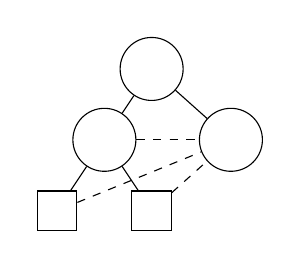
\begin{tikzpicture}[>=stealth,looseness=.5,auto]
\matrix [matrix of nodes,
  column sep={0.6cm,between origins},
  row sep={0.9cm,between origins},
  nodes={circle, draw, inner sep=1.3pt}]
  {
    & & \important{p}{} \\
    & \important{w}{} & & \important{w'}{} \\
    \leaf{u}{} && \leaf{v}{} \\
  };
  \tikzstyle{every node}=[font=\tiny\itshape]
  \draw (p) -- (w);
  \draw (p) -- (w');
  \draw[dashed] (w) -- (w');
  \draw (u) -- (w);
  \draw (v) -- (w);
  \draw [dashed] (u) -- (w');
\draw [dashed] (w) -- (w');
  \draw [dashed] (v) -- (w');
\end{tikzpicture}
\end{center}

\caption{A special quadruple .} \label{fig:quadruple}
\end{figure}


\begin{case}\label{case:70}
A leaf-sibling  of  that is not contained in a special quadruple has at least three requests to leaf siblings or nephews.
\end{case}

If  has at least three requests to leaf siblings , then we can branch by cutting  in the first side of the branch, and cutting all of  in the second side of the branch. This gives .

If  has two requests to nephews  and  such that  and  have the same parent  and , let  be a vertex other than  and  that  has a request to; if  is a nephew of  then favor it. Branch by cutting  in the first side of the branch, and cutting , one of , and  in the second side of the branch (note that since Case~\ref{case:2} does not apply, ). The reason why we can cut  in the second side of the branch follows from the fact that we would need to cut both  and  otherwise. This gives .

Finally, if the above does not apply, then we can favor all nephews of  that  has requests to, and branch by cutting  in the first side of the branch, and by cutting the siblings and nephews that  has requests to in the second side of the branch. This gives .

Now we can assume that for any important vertex , any leaf-sibling of  is either contained in a special quadruple, or has at most two requests to vertices in .


\begin{case}\label{case:7}
There exist two edges  and  in  such that all vertices  have cross requests.
\end{case}

Note that by Case~\ref{case:3}, each of  has exactly one cross request. Moreover, by Case~\ref{case:1.5}, if there is a cross request from any of  to an uncle, then the uncle is a leaf uncle.  Suppose that  has a cross request to ,  to ,  to , and  to . We distinguish the following subcases.

\begin{subcase}
\label{subcase:71}
Both  and  (or  and ) have requests to the same uncle (i.e.,  is a sibling of ).
\end{subcase}

Note that in this case  is a leaf uncle. Branch by cutting  in the first side of the branch, and keeping  and cutting  and the edges between  and the vertices of any minimum vertex cover of  in the second side of the branch (otherwise, if  is kept then both  and  would need to be cut). This gives .


\begin{subcase}
\label{subcase:72}
 and a vertex in , say , have requests to the same uncle, and  and  have requests to the same uncle (i.e.,  and , where both  and  are leaf uncles of ).
\end{subcase}
In this case the only requests involving  are , which can be cut by cutting three edges (e.g., cutting ). Note that if none of  is cut, then four edges are needed to cut the above requests; similarly, if two vertices in  are cut then four edges are needed to cut the above requests. Therefore, we can conclude that there exists a minimum cut that cuts exactly one vertex in  (if a minimum cut cuts two or more vertices from  then such a cut can be replaced by another cut of the same cardinality that cuts , , , and ; similarly if a cut does not cut any of ).  Branch by cutting  and the vertices of any minimum vertex cover of  in the first side of the branch, cutting  and keeping  and  in the second side of the branch, and cutting  and in the third side of the branch. This gives .



\begin{subcase}
\label{subcase:73}
Vertex  and a vertex in , say , have requests to the same uncle.
\end{subcase}


Since  is contained in some minimum vertex cover of , we can favor . Since any minimum vertex cover of  must contain either , ,
, or , by Lemma~\ref{lem:minvc}, there exists a minimum cut that either cuts  and , or  and , or  and , or  and . Therefore, we can branch in a 4-way branch by cutting  and  in the first side of the branch,  and  in the second side of the branch,  and  in the third side of the branch, and  and  in the fourth side of the branch. Since  are favored, in the first, second, and third sides of the branch  is kept. Observe the following. First, if a vertex in  has a request to a leaf uncle, then in any of the first three sides of the branch in which the vertex is not cut the uncle must be cut. Observe also that in the first side of the branch, if the two vertices  that are not cut have cross requests to two cousins , respectively, such that , then  can be cut (otherwise, both  and  need to be cut) in addition to one of ; if this is not the case then we can favor . Based on the above, the parameter is reduced by 4 in the first side of the branch, 4 in the second side of the branch, 4 in the third side of the branch, and 2 in the fourth side of the branch. We get
.


\begin{subcase}
\label{subcase:74}
No two requests from  go to the same uncle.
\end{subcase}

Similarly to Subcase~\ref{subcase:73}, we can favor two vertices in , chosen arbitrarily, say , and branch in a 4-way branch by cutting  and  in the first side of the branch,  and  in the second side of the branch,  and  in the third side of the branch, and  and  in the fourth side of the branch. Since  are favored, in the first, second, and third sides of the branch  is kept. By drawing the same observations as in Subcase~\ref{subcase:73}, we conclude that the first three sides of the branch result in a reduction of the parameter by a value of at least 4, whereas the fourth side of the branch results in a reduction of the parameter by a value of at least 2. We get .


The following proposition follows from the inapplicability of the above cases plus the fact that  is reduced:


\begin{proposition}
\label{prop:properties}
Let  be a reduced tree with root , and let  be an important vertex that is farthest from . If none of BranchRule~\ref{branch:1}, BranchRule~\ref{branch:3} and the above cases applies, then the following hold true:

\begin{itemize}

\item[(i)] For every child  of  (i.e., sibling of  or  itself) that is an important vertex,  consists of disjoint edges, length-3 paths, and cycles. No vertex that is contained in a cycle or a length-3 path in  has any cross requests, and every endpoint of an edge in  has at most one cross request.

\item[(ii)] For every child  of  that is an important vertex, there exist exactly two children  of  such that  and both  and  have cross requests.

\item[(iii)] Every leaf child   of  that is not contained in a special quadruple has at least one request, and at most two requests, to vertices in  that are either leaf siblings or nephews of .


\item[(iv)] Every non leaf child of  that is not contained in a special quadruple has no cross requests.
\end{itemize}
\end{proposition}

\begin{proof}

\begin{itemize}

\item[(i)] We know that . Therefore,  consists of disjoint paths and cycles. By part (v) of Proposition~\ref{prop:reduced},  contains no path of even length, and by BranchRule~\ref{branch:3},  contains no path of odd length . Therefore,  consists of disjoint edges, length-3 paths, and cycles. By Case~\ref{case:2}, no vertex in  of degree 2 has a cross request, and hence the only vertices in  that can have cross requests are endpoints of paths (or disjoint edges). By Case~\ref{case:2.5}, no endpoint of a length-3 path in  has a cross request, and hence no vertex of a length-3 path has a cross request. By Case~\ref{case:3}, no vertex in  has two cross requests, and hence every endpoint of a disjoint edge has at most one cross request. The statement follows.

\item[(ii)] By part (i) above, the only vertices in  that can have cross requests are endpoints of disjoint edges. By part (vii) of Proposition~\ref{prop:reduced}, there is no minimum vertex cover of  that cuts all cross requests. Therefore, there must exist at least one disjoint edge in  whose both endpoints have cross requests. By Case~\ref{case:7}, such an edge must be unique. The statement follows.

\item[(iii)] The fact that a leaf child of  must have at least one cross request follows from part (ii) (and part (i)) of Proposition~\ref{prop:reduced}. By Case~\ref{case:70}, no leaf child of  that is not contained in a special quadruple can have more than 2 cross requests. The statement follows.

\item[(iv)] Let  be a non leaf child of  that has a cross request to a vertex , and we show that  must be contained in a special quadruple. By Case~\ref{case:0}, the cross request from  must be to a leaf sibling. By Case~\ref{case:4}, the size of a minimum vertex cover of  is exactly 1 (note that every vertex in  has degree at least 1), and hence  consists of a single edge . By part (ii) of the current proposition, both  and  have cross requests, and by Case~\ref{case:1.5}, the requests from  and  must be to leaf uncles. Also, by Case~\ref{case:3}, each of  and  has exactly one cross request. By Case~\ref{case:5},  must have exactly one cross request to  and the cross requests from both of  and  must be to . Finally, by Case~\ref{case:6}, the cross requests from  must be only to , , and . The statement follows.

\end{itemize}
\end{proof}


\begin{definition}\rm
\label{def:auxiliary1}
Let  be a reduced tree with root , and let  be an important vertex that is farthest from . Suppose that none of BranchRule~\ref{branch:1}, BranchRule~\ref{branch:3}, or the above Cases applies. We define the auxiliary graph  as follows. The vertices of 
are the leaf children and the grandchildren of  that are not contained in any special quadruple.  Two vertices  and  in  are adjacent if and only if . Note that the edges in  correspond to either a request between two grandchildren of  that have the same parent, a request between two leaf children of , or a request between a leaf-child and a grandchild of .
\end{definition}


The following proposition is the dual of Proposition~\ref{prop:reduced}:

\begin{proposition}
\label{prop:propertiesbranching}
Let  be a reduced tree with root , and let , where , be an important vertex that is farthest from . Suppose that none of BranchRule~\ref{branch:1}, BranchRule~\ref{branch:3}, or the above Cases applies. Consider the graph . Then the following are true:

\begin{itemize}
\item [(a)] , and hence  consists of disjoint paths and cycles.

\item[(b)] For every path  in  such that at least one endpoint of  is a grandchild of , there exists a minimum cut that cuts the vertices in some minimum vertex cover of .


\item[(c)] For every path  and every cycle  in , there exists a minimum cut  such that the number of edges in  that are incident on the vertices in  or their parents in case these vertices are grandchildren of , is equal to the size of a minimum vertex cover of , and the number of edges in  that are incident on the vertices in  or their parents in case these vertices are grandchildren of , is equal to the size of a minimum vertex cover of .

\end{itemize}
\end{proposition}

\begin{proof}

Part (a) follows from parts (i), (ii), (iii) of Proposition~\ref{prop:propertiesbranching}.

Parts (b) and (c) are similar to Lemma~\ref{lem:minvc} in spirit. Proving them, however, is more subtle since a minimum cut can cut an important vertex, which would cut all cross requests from its children, and important vertices are not vertices of .


Consider a minimum cut  of . Call a path in  whose both endpoints are leaf children of  a {\em type-I path}, and a path with at least one endpoint that is a grandchild of  a {\em type-II path}.

To prove part (b), consider a type-II path  in . It is not difficult to see that any cut to  must cut at least  (the size of a minimum vertex cover of ) many vertices of . Moreover, for every vertex of , all its requests to vertices in  are to vertices on . Therefore, if  cuts more than  many vertices from , then the vertices of  that are cut by  can be replaced by those in a minimum vertex cover of  plus vertex ; this will result in a minimum cut of  that cuts exactly  many vertices from . Therefore, we can assume that  cuts precisely  vertices from , and it suffices to show that the vertices of  that are cut by  can be replaced by a vertex cover of .


Suppose that , where  is a grandchild of , and let  be the set of vertices in  that are grandchildren of ; note that . If  does not cut any parent of a vertex in , then it can be readily seen that the vertices of  that are cut by  must form a vertex cover of  (those vertices would consist only of grandchildren and leaf children of , and hence of vertices of ). Suppose now that  cuts al least one parent of a vertex in . Suppose first that  cuts the parent of a vertex  such that  is not an endpoint or a sibling of an endpoint of ; let  (note that in this case ). Let  be the child of  such that . By part (ii) of Proposition~\ref{prop:properties}, the edge  does not cut any request on a type-I path or a cycle in  because  are the only children of  that both have cross requests and such that . Therefore, the edge  only cuts type-II paths of the form  where both  and  are children of . For each such path , if  contains  then swap it with ; we still get a minimum cut, say  without loss of generality, such that  cuts all requests on type-II paths of the form   where  and  are children of . Repeating the above for each such vertex , and replacing the edges in  that are incident on vertices of  with edges that are incident on some minimum vertex cover of , and replacing edge  in  with edge , yields a minimum cut that cuts the vertices in a minimum vertex cover of .

We can assume now that  cuts the parent of an endpoint of , say . Then  does not cut any parent of a vertex  in , and  must cut a vertex cover of the subpath . Moreover,  must cut either  or . If  cuts  then replace  with  to obtain a minimum cut that cuts a minimum vertex cover of ; otherwise,  cuts a minimum vertex cover of . The case is similar if  cuts an endpoint of  that is a leaf child of . This proves part (b).


To prove part (c), consider a type-I path or a cycle in . Observe that by part (a) above and by part (ii) of Proposition~\ref{prop:properties}, no edge in  that cuts a request on a type-I path or a cycle in  cuts any other request on a type-I path or cycle. (Note that its is possible that an edge that cuts a request on a type-I path or cycle cuts a request on a type-II path. However, this will not affect the fact that  cuts exactly the size of a minimum vertex cover many vertices from every type-II path). Therefore, if  cuts more than  many vertices from a type-I path  in , or more than  from a cycle  in , then those vertices that are cut by  can be replaced by the vertices in a minimum vertex cover of  or , plus vertex , to yield a minimum cut of  that cuts exactly  many vertices from every path  and  many vertices from every cycle  in . This completes the proof.
\end{proof}


The following reduction rule follows from parts (b) and (c) of Proposition~\ref{prop:propertiesbranching} after noticing that for a path of even length, there is a unique set of edges of cardinality  in  that cuts all requests corresponding to the edges of :

\begin{reduction}\label{red:10}
Let  be a reduced tree with root , and let  be an important vertex that is farthest from , and such that . Suppose that none of BranchRule~\ref{branch:1}, BranchRule~\ref{branch:3}, or the above Cases applies. If there exists a path  in  of even length then cut the vertices in  that correspond to the unique vertex cover of .
\end{reduction}


The following branching rule follows from parts (b) and (c) of Proposition~\ref{prop:propertiesbranching}, after noticing that for a path of odd length in , there is a unique set of edges of cardinality  in  that cuts all requests corresponding to the edges of  in addition to cutting an endpoint of :

\begin{branchrule}\label{branch:4}
Let  be a reduced tree with root , and let  be an important vertex that is farthest from , and such that . Suppose that none of BranchRule~\ref{branch:1}, BranchRule~\ref{branch:3}, or the above Cases applies. If there exists a path  in  of odd length such that , let  be an endpoint of  and let  be the (unique) minimum vertex cover of  containing . Branch by cutting the vertices in  and contracting the edges between  and vertices in  in the first side of the branch, and by cutting the neighbor of  in  in the second side of the branch. Since ,  satisfies the recurrence relation: .
\end{branchrule}


The following branching rule follows from parts (b) and (c) of Proposition~\ref{prop:propertiesbranching} after noticing that, for a cycle of even length in  there are exactly two sets of edges in , each of cardinality , such that each cuts all requests corresponding to the edges of :

\begin{branchrule}\label{branch:5}
Let  be a reduced tree with root , and let  be an important vertex that is farthest from , and such that . Suppose that none of BranchRule~\ref{branch:1}, BranchRule~\ref{branch:3}, or the above Cases applies. If there exists a cycle  in  of even length, branch into a two sided branch: in the first side of the branch cut the vertices corresponding to one of the minimum vertex covers of , and in the second  side of the branch cut the vertices corresponding to the other minimum vertex cover of .  Since , and hence , we get .
\end{branchrule}


\begin{branchrule}\label{branch:5}
Let  be a reduced tree with root , and let  be an important vertex that is farthest from , and such that . Suppose that none of BranchRule~\ref{branch:1}, BranchRule~\ref{branch:3}, or the above Cases applies. If there exists a cycle of odd length  in  such that  and  is not a cycle in  for some child  of , then branch as follows. First observe that since  is not a cycle in  for some child  of ,  is odd, and  is reduced, at least one vertex, say  on  must be a leaf child of . We favor the vertices in  that are grandchildren of  (if any). In the first branch  is kept and  are cut. In the second side of the branch  is cut, and the cycle becomes a path of odd length at least 5; therefore, we can further branch according to BranchRule~\ref{branch:4}. This yields .
\end{branchrule}


Now let  be a reduced tree with root , and let  be an important vertex that is farthest from , and such that . Suppose that none of the branching rules of the above cases applies. Then each vertex in  is contained in one of the following structures/groups in . Group I, abbreviated , are paths of length 1 (edge) in  between two children of an important child of , Group II, abbreviated , are paths of length 1 in  between two leaf children of , Group III, abbreviated , are paths of length 3 in  but not in  for any important child of , Group IV, abbreviated  are cycles of length 3 in  but not in  for any important child of , Group V, abbreviated , are cycles of lengths 5 in   but not in  for any important child of , Group VI, abbreviated  are special quadruples, and Group VII, abbreviated , are paths of length  or cycles in , for some important child  of . Note that no vertex in  can have a cross request. The structure of the groups are illustrated in Figures~\ref{fig:1}~--~\ref{fig:6}, in addition to Figure~\ref{fig:quadruple}.

\include{figures}

Let , and let  be the siblings of . Each sibling  of  is either a leaf, an important vertex, or  has a similar structure to .

\begin{case}
\label{case:100}
If for any , there is no request from a vertex in  to a vertex in some tree , for any , then contract the edge between  and its parent.
\end{case}
This can be seen as follows. If  is cut by some minimum cut , then since there are no requests between vertices in  and a vertex in , for any  in , edge  can be replaced by the edge between  and its parent to yield a minimum cut that excludes the edge between  and its parent. Therefore, we can assume that, for any , there exists a request between some vertex in  and a vertex in some . Moreover, for any vertex  in , there exists a minimum cut that cuts . Further, if any edge  on the path between  and  is part of a minimum cut, then there is a minimum cut that includes  and cuts  as well. Therefore,  can be favored in the sense that if  is kept in a certain branch then all edges on the path between  and  are kept as well.


Consider now  for some fixed . Let  be a vertex in  that has a request to a vertex  in , for some . We favor both  and .  We distinguish the following cases.

\begin{case}
\label{case:200}
 is an important vertex. We can branch with .
\end{case}

Since  is important,  must have two children  such that  and both  and  have cross requests. Suppose that  has a cross request to  in . Favor  (if  is a grandchild of ) and . Branch by cutting  in the first size of the branch and keeping , and by cutting  in the second side of the branch. In the first side of the branch  is kept and so is . Therefore,  and  must be cut. This gives .

We can assume now that  is not an important vertex in . Therefore,  must be a vertex in ; let  be the degree of  in .

\begin{case}
\label{case:300}
.  We can branch with .
\end{case}


If in a certain branch  is kept, then two edges can be cut. This can be seen as follows. If  is a  vertex, then both neighbors of  in  can be cut (favor the neighbors that are not leaf children of ). If  is a  vertex, let  be the length-3 cycle containing .  If  is a leaf child of , then the parent of  can be cut, in addition to one of  (chosen arbitrarily). If  is not an leaf child of , then  and  can be cut (since  is favored). If  is a  vertex, then by favoring any neighbor of  in  that is not a leaf child of  (if the neighbor is a leaf child of  then there is no need to favor it), it can be easily seen that when  is kept then its two neighbors can be cut. If  is a  vertex, then the same analysis carries as when  is  vertex. Finally, if  is a  vertex, then it can be easily seen that both neighbors of  can be cut.

Therefore, if , then we can branch by cutting  in the first side of the branch, and keeping  and cutting its two neighbors in , in addition to  in the second side of the branch. This gives .

\begin{case}
\label{case:400}
Suppose now that  in . We can branch with .
\end{case}

In this case either  is a  or a  vertex that is an endpoint of a length-3 path, or  is a  or a  vertex . If  is an endpoint of a length-3 path , then by part (b) of Proposition~\ref{prop:propertiesbranching}, if  is cut, then  must be cut as well. On the other hand, if  is kept then  and  must be cut. This gives .

We can now assume that all requests between the 's go from  or  vertices to  or  vertices.

\begin{case}
\label{case:500}
 is an endpoint of a  group. We can branch with .
\end{case}


If  is an endpoint of a  group, let , and let  be the child of  such that .  Note that  is an important vertex, and hence, there exists , children of , such that  and both  and  have cross requests. We favor  and branch as follows. In the first side of the branch we cut  and keep , and in the second side of the branch we keep  and cut . Let us analyze the second side of the branch when  is kept. In this case  must be cut. Since  is kept and is favored,  is kept as well. Since both  and  have cross requests,  and  are either part of a , , , or  group. If  and  are contained in a  or a  group, then their uncle must be cut leading to a further reduction of the parameter by at least 1. If  and  are contained in a  group , then by part (b) of Proposition~\ref{prop:propertiesbranching} either  or  must be cut, so we can branch further into these two branches. If  and  are part of a  group , where  and  are children of an important child of , then since  is kept we branch on : if  is cut, then  is kept and  is cut (since  is kept), and if  is kept then  and  are cut. In the worst case, we get .

\begin{case}
\label{case:600}
All requests between the 's go between  vertices. We can branch with .
\end{case}

If for every  group in  at most one vertex has a request to some , where , then there exists a cut of  that cuts all requests to , and whose cardinality is equal to the set of edges in a minimum cut that are contained in ; therefore, edge  can be contracted.  Hence, we can assume that for every , there exists a  in  whose both vertices  have requests to vertices in other trees; suppose that  has a request to  and  to , where  and  are not in . Moreover, we can assume that  contains an important vertex (choose a tree among the 's that contains an important vertex, and by the above argument, there exists a  in  whose both vertices  have requests to vertices in other trees). Since each important vertex must have two children with cross requests, and since there is a  in , any minimum cut must cut at least three vertices in . We branch as follows. Either  is cut or is kept. When  is cut, at least 3 edges in , corresponding to any minimum cut of  can be cut. When  is kept, we branch by cutting  and favoring  in the first side of the branch, and cutting  and favoring  in the second side of the branch. When  is cut,  is kept, and hence  must be cut (since  is kept). When  is cut,  is kept and hence  is cut. This gives .


\begin{theorem}
\label{thm:main}
The MCT problem is solvable in time , where .
\end{theorem}

\begin{proof}
The above cases exhaust all possible scenarios. The worst branch is , which corresponds to the characteristic polynomial  whose positive root is  . It follows that the running time of the algorithm is , where .
\end{proof}


\section{The GMWCT problem}
\label{sec:gmwct}
There is a simple reduction from GMWCT to MCT.  For an instance  of GMWCT, construct the instance , where the set of requests  is given as follows. For each terminal set , , and for every pair of distinct terminals , add the request  to . Clearly,  is a yes-instance of GMWCT if and only if  is a yes-instance of MCT.
Combining this reduction with Theorem~\ref{thm:main} we obtain:

\begin{theorem}
\label{thm:gmwct}
The GMWCT problem is solvable in time , where .
\end{theorem}




\subsection{A linear time algorithm for WGMWCT}
\label{subsec:wgmwc}
Next, we show that the GMWCT problem is solvable in linear time when the number of terminal sets is a constant. (Clearly, the problem is NP-complete when the number of terminal sets is part of the input by a simple reduction from the MCT problem.) The algorithm is a dynamic programming algorithm that solves the more general weighted version of the problem, denoted WGMWCT, defined as follows: Given a tree  in which each edge is associated with a nonnegative cost , and terminal sets , where  is a constant, compute a minimum-cost set of edges
whose removal cuts each pair of distinct terminals in , for .

{\bf Assumptions.}
First of all, root the input tree  at {\em any} vertex.
Let  be the root of . We first apply some simple preprocessing:
\begin{enumerate}
\item If an internal vertex  is a terminal, we can add a child of , say , and assign the edge  a large enough cost; then replace each appearance of  in collection  by .
All leaves that are {\em not} terminals can be removed from the tree. After this preprocessing, we may assume that {\em a vertex  is a leaf if and
only if  is a terminal}.

\item If a vertex  has more than  children, then we can replace  by a chain of  vertices connected by a path in which each edge has a large enough cost. The original children of  is then connected to the vertices in the chain so that each vertex in the chain has two children. After this preprocessing, we may also assume that {\em the input tree  is a binary
tree}.
\end{enumerate}

{\bf Basic idea.}
Our approach to solve WGMWCT is dynamic programming, based on the following
simple observation. When an optimal multiway cut is removed from the input
tree ,  is broken into several subtrees. In each subtree, there is
at most one terminal for {\em every} terminal set  (), and
there must be at least one terminal which comes from {\em some} terminal set.


{\bf The algorithm.}
Let  be a vertex in the tree  and  the subtree of  rooted at . When certain edges are removed in , some terminals in the original 
are still connected to  and some terminals are not. We use a binary vector  to record the {\em connection pattern} of the tree, where  () if there exists exactly one terminal from
 that is connected to  and  if there is no terminal from  that is connected to  (if two or more terminals from  are connected to , then the cut is invalid). Denote by  the minimum cost of edges whose removal makes  satisfy . If such a set of edges does not exists,  is defined to be . The goal of the algorithm is to compute  for all vertices  and all binary vectors .

We consider three cases:

{\bf Case 1.  has two children  and .} We will compute  based on the assumption that  and 
have already been computed. Let  be connection patterns of  and  respectively, and let  be a subset of . If  has connection pattern  after the edges in  are removed, we say that  is {\em derived from} the tuple , denote by 

We have the following recurrence relation:


Although there are  possible tuples
, less number of tuples need to be considered when computing :

If  (i.e., both  and  are removed), then  regardless of  and . So we only need to consider one tuple , where  is minimum among all  and  is minimum among all .

If  (i.e.,  is removed), then  regardless of . So we only need to consider  tuples , where  is minimum among all . Similarly, if , only  tuples are considered.

If  (neither edge is removed), then the two vectors  and  cannot both have 1 at the same position  because this would imply  has two terminals in . Therefore each position  has only three possible pairs of values in the two vectors: (0,0) (1,0), and (0,1). In other words, only  tuples are considered.

Therefore, for any vertex , it takes time  to compute  for all .

{\bf Case 2.  has only one child .} Similar to the above, we have the following recurrence relation:

In this case, it takes time  to compute  for all .

{\bf Case 3.  is a leaf.} By our assumption,  must be a terminal. We say that the vector  is valid if  () if and only if .
The formula for computing  is

In this case, it takes time  to compute  for all .


We can compute  for all vertices  in the tree  in a bottom-up manner.
The optimal value  is equal to
. By backtracking, we can recover the optimal solution achieving
. Since the computation at any given vertex  takes time , the total running time of our dynamic programming algorithm is
, which is linear in  because  is a constant.
Thus we have
\begin{theorem}
\label{th - GMWCT can be solved in linear time}
The Generalized Multiway Cut problem on trees can be solved in linear time.
\end{theorem}

\section{Concluding remarks}
\label{sec:conclusion}
In this paper we gave a parameterized algorithm for the {\sc MCT} problem that runs in time , improving the previous algorithm by Chen et al. that runs in time . The aforementioned result implies that the {\sc GMWCT} problem is solvable in time  as well. We also proved that the special case of the {\sc GMWCT} problem in which the number of terminal sets is fixed is solvable in linear time, answering an open question by Liu and Zhang~\cite{LZ12}.

There are several questions related to the problems under consideration that remain open and are worth pursuing. First, it is interesting to seek further improvements on the running time of parameterized algorithms for the {\sc MCT} and the {\sc GMWCT} problems. The {\sc vertex cover} problem admits a parameterized algorithm that runs in time ~\cite{ckj}, and one can ask if the connection between {\sc MCT} and {\sc vertex cover} can be exploited further to improve the running time of parameterized algorithms for {\sc MCT} further. Another interesting research direction is related to kernelization. Currently, {\sc MCT} is know to admit a kernel of size ~\cite{multicut}, and it is interesting to investigate if the problem admits a quadratic, or even a linear, kernel. The  kernel for {\sc MCT} relies heavily on kernelization techniques used for {\sc vertex cover}. So again, it would be interesting to investigate if one can exploit this connection further to obtain improvements on the kernel size for the {\sc MCT} problem. We leave those as open questions for future research.


\bibliographystyle{plain}
\bibliography{ref}



\end{document}
